\documentclass[dvipdfmx]{ujarticle}
\usepackage[dvipdfmx]{graphicx}
\setlength{\textwidth}{170mm}
\setlength{\textheight}{260mm}
\setlength{\oddsidemargin}{-5mm}
\setlength{\topmargin}{-25mm}

\title{単一QD-SOAを用いた全光XOR-AND回路}
\author{}

\begin{document}
\maketitle

\section{はじめに}
近年のインターネット通信端末の増加と普及により,光通信による通信の高速化と大容量化が必要不可欠となっている.
現在の光通信では,信号処理を行う際に一度光信号から電気信号へと変換するため通信速度の最大値が電気信号の処理速度に依存してしまうという課題がある.
従って電気信号への変換処理が必要ない全光信号処理技術を構成する全光論理回路の研究が進められている.
従来研究として実装されている全光論理回路の多くは光がデバイスに入射した際に発生する非線形光学効果を利用している.
その中でも量子ドット半導体光増幅器(Quantum-Dot Semiconductor Optical Amplifiers: QD-SOA)を用いた全光論理回路が提案されている.
QD-SOAは量子ドット構造の活性層を持つ光増幅器のことであり,電子を量子ドット内に閉じ込めることで従来の光増幅器よりも大きな利得を得ることができる.
従来研究として提案されている全光XOR回路ではマッハ・ツェエンダー干渉系(Mach-Zehnder Interferometer:MZI)を用いた回路が提案されている.
しかし,MZIを用いた全光回路は同一特性のQD-SOAを2つ使用しなければならないが同一特性のQD-SOAを製造することは非常に困難という問題がある.
上記の問題点を踏まえて本研究ではMZIを用いない単一のQD-SOAで動作する全光XOR-AND回路を提案し, シミュレーションによる性能評価を行う.

\section{単一QD-SOAを用いた全光XOR-AND回路}

\begin{figure}[h]
  \begin{center}
    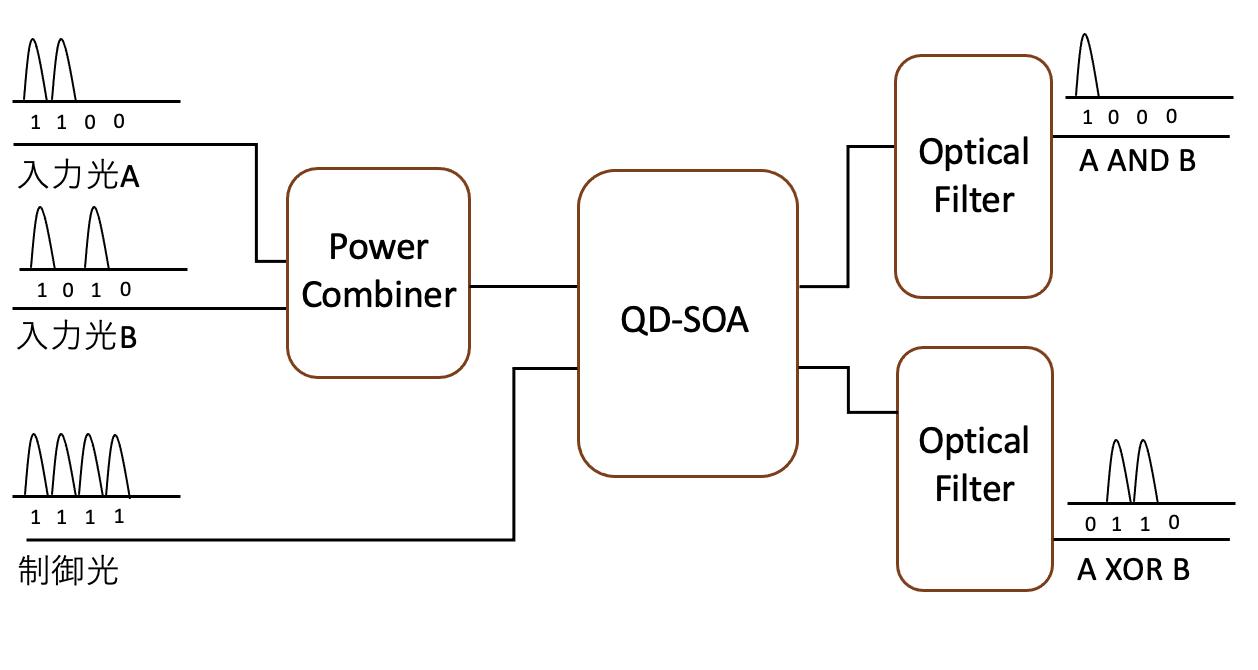
\includegraphics[width=15cm]{kairo2.png}
    \caption{提案する全光XOR-AND回路の構成}
  \end{center}
\end{figure}
提案する全光回路ではまず, 入力光A,Bを複数の光を合波するデバイスであるPowerCombiner(PC)に入射させる.
その後合波された光と制御光を入力としたQD-SOAで光を増幅させ,最後に特定の波長の光を取り出すデバイスであるOptical Filter(OF)から基本論理回路として必要な波長のみを取り出し最終的な出力光とする.

\section{シミュレーション}
\subsection{条件及び評価指標}
本研究では OptiSystem16.1.0, MATLAB 2019a を用いてシミュレーションを行った.
QD-SOAは光の伝搬方程式, キャリアのレート方程式及び伝達行列法(Transfer Matrix Method:TMM)を用いてシミュレーションを行う.
光の伝搬方程式はQD-SOA内の光電界に関する式であり,キャリアのレート方程式はQD-SOA内の時間変化によるキャリアの変化を表す式である.
また,伝達行列法はQD-SOAを光の伝搬方向に対して細かく分割しキャリア密度, 光子密度, 利得を繰り返し求めることで結果的に出力される光電界を求める手法である.
今回シミュレーションで使用するパラメータは表1に示したものを用いた.\\
シミュレーションでは入力光強度と各論理回路に対応する光フィルタの指定波長を変化させ、それぞれの条件に対する消光比が最も高くなるようなパラメータ探索を行う.

\begin{table}[h]
  \caption{シミュレーションで用いるパラメータ}
  \centering
    \begin{tabular}{ccc}
      \hline
      パラメータ名 & 値 & 単位 \\
      \hline
      QD-SOAの長さ & $ 3.0 \times 10^{-3} $ & $m$\\
      QD-SOAの厚さ & $ 0.25 \times 10^{-6} $ & $m$\\
      QD-SOAの幅 & $ 3.0 \times 10^{-6} $ & $m$\\
      量子ドット密度 & $ 5.0 \times 10^{14} $ & $m^{-2}$\\
      キャリア寿命(WL→ES) & $ 3.0 \times 10^{-12} $ & $s$ \\
      キャリア寿命(ES→WL) & $ 1.0 \times 10^{-9} $ & $s$\\
      キャリア寿命(WL→系外) & $ 2.0 \times 10^{-9} $ & $s$\\
      キャリア寿命(ES→GS) & $ 0.16 \times 10^{-12} $ & $s$\\
      キャリア寿命(GS→ES) & $ 1.2 \times 1o^{-12} $ & $s$\\
      キャリア寿命(GS→系外) & $ 0.4 \times 10^{-9} $ & $s$\\
      注入電流 & $5.0 \times 10^{-2}  $ & $A$\\
      \hline

    \end{tabular}
\end{table}

\subsection{評価指標}
評価指標としてアイダイアグラム(eye diagram)および消光比(Extinction Ratio: ER)を用いる.
アイダイアグラムとは信号光を1ビット幅間隔で分割し,重ね合わせて描画したグラフのことであり,
消光比は ${P^1}_min$を"1"として出力された光の中で最も強度が弱いときの光強度の値,
${P^0}_min$を"0"として出力された光の中で最も強度が強い時の光強度の値としたときに
$ER[dB] = 10 \log{10}{\frac{{P^1}_min}{{P^0}_max}}$ で算出される指標である.
この値が大きいほど出力光が"0","1"の区別がつきやすい優れた波形であることを示す.

\subsection{シミュレーション結果}
AND演算およびXOR演算を行った場合のシミュレーション結果をアイダイアグラムの形で描画すると以下のように表せる.
AND演算における消光比は14.89dB, XOR演算における消光比は10.21dBが得られた.

\begin{figure}[h]
  \begin{center}
    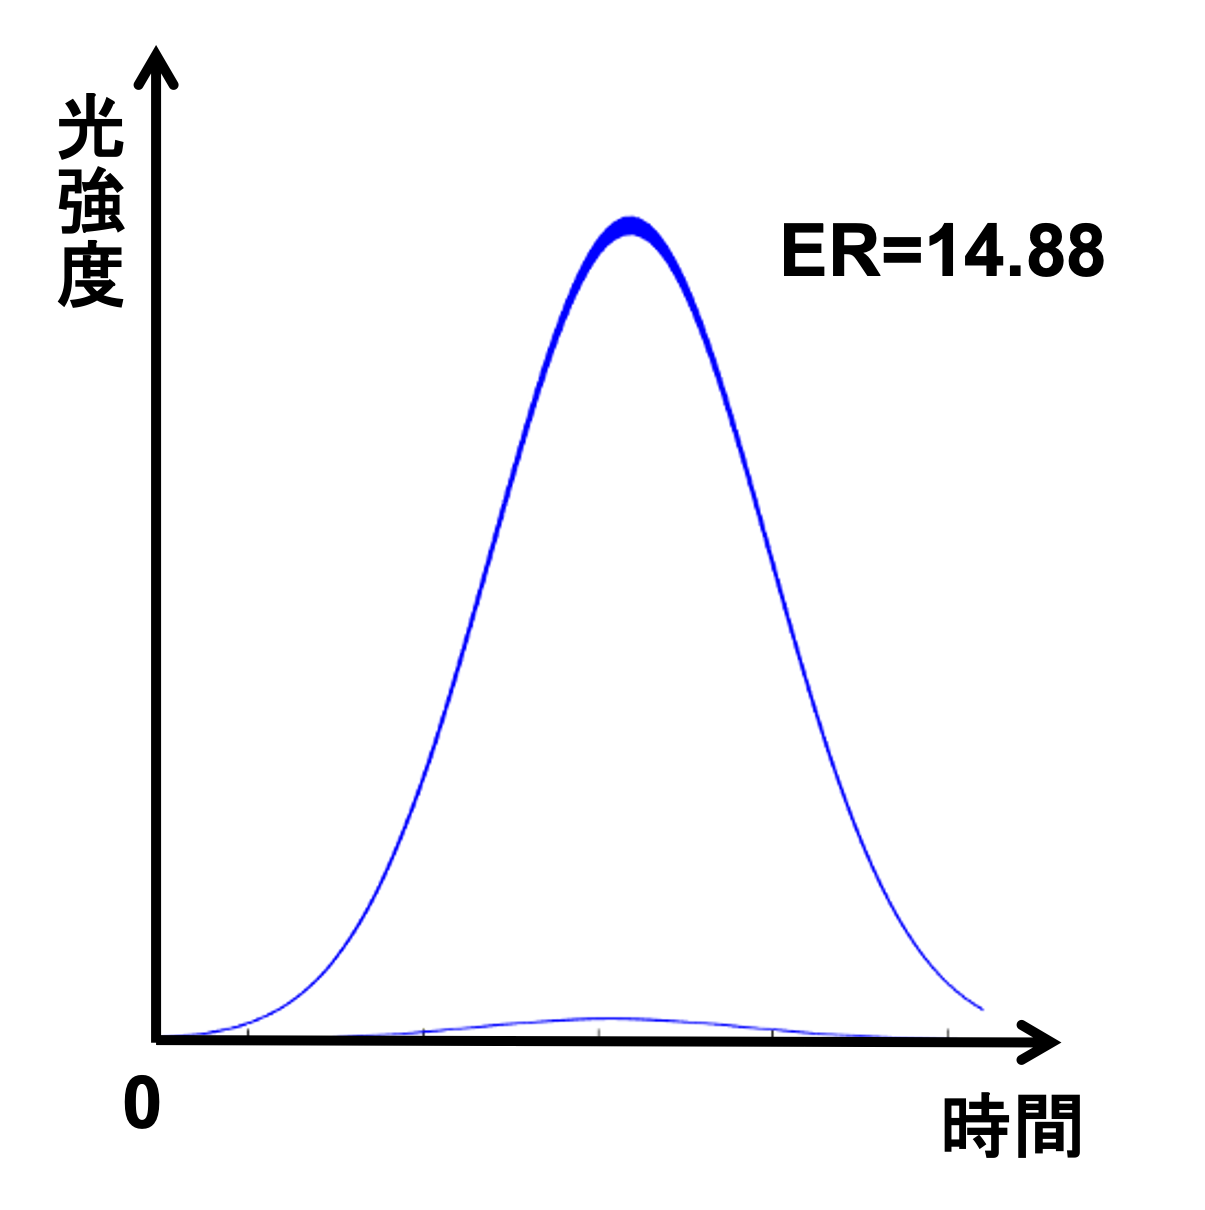
\includegraphics[width=5cm]{images/and_result.png}
    \caption{AND回路の結果}
  \end{center}
  \begin{center}
    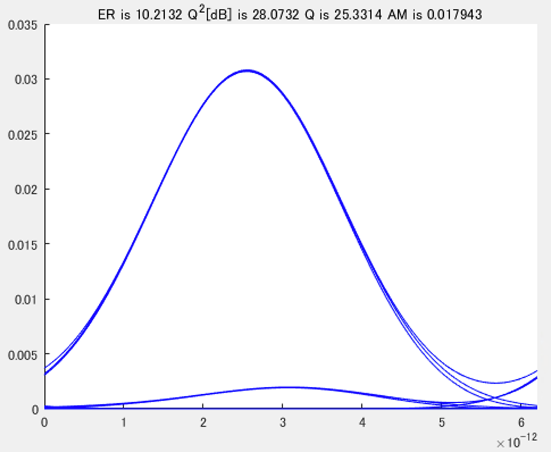
\includegraphics[width=5cm]{images/xor_result.png}
    \caption{XOR回路の結果}
  \end{center}
\end{figure}

\section{まとめ}
単一QD-SOAを用いた全光AND/XOR論理回路を提案した.
シミュレーション結果より論理回路の動作を確認でき, 評価指標から出力波形の品質は良好と見られる.
今後の課題としてはQD-SOA内で発生する雑音を考慮したシミュレーション結果の検討やパラメータの最適化が挙げられる.


\end{document}
